\documentclass{article}
\usepackage[left=3cm,right=3cm,top=3.5cm,bottom=2cm,
bindingoffset=5mm]{geometry}
\usepackage[utf8]{inputenc}
\usepackage[T1]{fontenc}
% Fuente escalable
\usepackage{lmodern}
\usepackage[english,spanish]{babel}
\usepackage{amsmath}
\usepackage{amssymb,amsfonts,textcomp}
\usepackage{array}
\usepackage{supertabular}
\usepackage{booktabs}
\usepackage{threeparttable}
\usepackage{hhline}
\usepackage[pdftex]{graphicx}
\usepackage{microtype}
% Bibliografia
%\usepackage{bibtex}
\usepackage{biblatex}
\bibliographystyle{amsplain}
\bibliography{Bibliografia.bib}
% Formato de unidades
\usepackage{siunitx}

% Graficos
\usepackage{tikz}
% Esquematicos
\usepackage[siunitx, american, cuteinductors, smartlabels]{circuitikz}
% Tablas con ancho establecido por usuario
\usepackage{tabularx}
% Agrega comandos extra al comando tabular
% \toprule, \midrule, \bottomrule
\usepackage{booktabs}
% Permite unir varias filas en tablas
\usepackage{multirow}
% Encabezados personalizados
\usepackage{fancyhdr}
\usepackage{graphicx}

\makeatletter
\newcommand\arraybslash{\let\\\@arraycr}
\makeatother
\setlength\tabcolsep{1mm}
\renewcommand\arraystretch{1.3}
\newcounter{Table}
\renewcommand\theTable{\arabic{Table}}
\newcounter{Drawing}
\renewcommand\theDrawing{\arabic{Drawing}}
\title{}
\author{}
\date{2017-03-28}

% Cabeceras
\pagestyle{fancy}
% Borra cabecera y pie actuales
\fancyhf{}
% Cintillo cabecera
\chead{
	
\includegraphics[width=150mm]{Imagenes/Cabecera.png}
}

\begin{document}
	\title{\textsc{Sistema para Medicion de Figura de Ruido}} 
	\author{Jose A. Arias B.}
	\date{28-03-2017}
	% Comando para imprimir el encabezado(titulo, subtitulo, autor, fecha=
	\maketitle
	\clearpage
	
	% Crea pagina de titulo
%	\begin{titlepage}
%		% \vspace Inserta espacio vertical 
%		% \vspace*{dimnesion} fuerza insercion espacio vertical
%		\vspace*{1cm}
%		% \par Finaliza parrafo
%		{\huge\raggedright \textsc{Sistema para Medicion de Figura de Ruido}\par}
%		% \hrule crea linea horizontal
%		% \noindent elimina sangria primera linea
%		\noindent\hrulefill\par
%		{\LARGE\raggedleft Jose Arias\par} 
%		% Inserta espacio vertical comprimible
%		\vfill 
%		{\Large\raggedleft Cendit\par}		
%	\end{titlepage}	
	
	% Genera la tabla de contenidos
	\tableofcontents
	
	\clearpage
	
	\section{Informe descriptivo del banco para pruebas con fuente de ruido}
	\subsection{Introducción}
	La presente obra es un informe descriptivo del banco para medición de figura de ruido presente en la Fundación CENDIT.
	Este sistema esta constituido casi en su totalidad por equipos de Agilent Technologies, es descrito en una nota de	aplicación como un sistema destinado a pruebas con fuentes de ruido, entre ellas, su calibración.
	
	\subsection{Objetivo}
	Por medio de una descripción general del sistema y una descripción de carácter técnico de cada uno de sus componentes, se pretende lograr un visión general acerca del uso y situación actual del banco de medición de figura de ruido dentro del CENDIT.
	
	\subsection{Descripción general del sistema}
	En un resumen técnico de la empresa Agilent Technologies \cite{AGI01} se propone los equipos mostrados en la \ref{Fig:BancoPruebasFuenteRuido} como un sistema para realizar pruebas con fuentes de ruido, entre ellas su calibración, para aplicaciones de radio frecuencia
	(RF) y microondas (UW). De acuerdo a esta nota técnica, el sistema planteado estaría compuesto por tres equipos
	fundamentales de Agilent Technologies, asociados con equipos periféricos de interconexión y apoyo.
	
	\begin{itemize}
		\item Un analizador de figura de ruido, modelo N8975A.
		\item Un controlador de interruptores y atenuadores, modelo 11713A.
		\item Un banco de atenuadores y aisladores, modelo N2002A.
	\end{itemize}	

	\begin{figure}[h!]
		\begin{minipage}{16.009cm}					
			\centering
			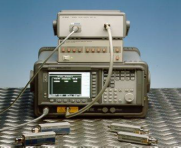
\includegraphics{Imagenes/BancoPruebasFuenteRuido.png}
			\caption{Banco para pruebas con fuentes de ruido, propuesto por Agilent Technologies}
			\label{Fig:BancoPruebasFuenteRuido}
		\end{minipage}
	\end{figure}

	El sistema incluye además fuentes de ruido, cables de interconexión y adaptadores coaxiales, algunos de los cuales se aprecian en la figura \ref{Fig:BancoPruebasFuenteRuido}.
	
	Si la caracterización de fuentes de ruido bien puede realizarse con un analizador de figura de ruido, como el equipo N8975A de la figura \ref{Fig:BancoPruebasFuenteRuido}, la empresa Agilent sugiere emplear dos dispositivos adicionales, si se desea disponer de la instrumentación adecuada para calibración de fuentes de ruido con elevada exactitud y trazabilidad. 
	
	De acuerdo a Agilent, un factor que degrada la exactitud y aumenta la incertidumbre en las mediciones de parámetros de ruido, es la interacción que existe a la salida de la NS y la entrada de señal del NFA, debida a ligeros desacoples de impedancia. Se emplearían entonces un banco de aisladores y atenuadores, el dispositivo Agilent N2002, interpuesto en el camino de señal, entre la salida de la fuente de ruido y la entrada del NFA, con el objeto de disminuir la interacción entre la NS y NFA para asi lograr medidas de elevada exactitud y baja incertidumbre.
	
	Como dispositivo N2002 no presenta interfaz de usuario ni posee “inteligencia” interna que permita comandarlo, requiere de un dispositivo controlador externo, un equipo de la serie 11713 de Agilent. Por medio de la interfaz que dispone el 11713, el usuario realiza la selección de la atenuación requerida en el banco de atenuadores N2002A.
	
	Las mediciones de potencia de ruido en dispositivos RF y UW exige fuentes de ruido calibradas si se desea una elevada precisión y exactitud, el error en dichas mediciones esta fuertemente ligado a la incertidumbre de la fuente de ruido	empleada. Por ello es de vital importancia su calibración, entendida esta como la verificación que se realiza en los	parámetros de la fuente de ruido para asegurar que la misma se encuentra dentro de los valores nominales establecidos	por la calibración de fabricante. 
	
	Por medio del sistema propuesto por Agilent, se puede calibrar las fuentes de ruido “en casa”, sin depender de laboratorios de calibración externos.
	
	Uno de los pasos en el proceso de calibración de fuentes de ruido es la medición de la razón de ruido en exceso |\textit{ENR} (\emph{Excess Noise Ratio}) de la fuente en cuestión. Si bien este paso de la calibración puede realizarse empleando únicamente un analizador de figura de ruido, la motivación de Agilent al presentar este sistema es que utilizando los dispositivos N2002A y 11713A en conjunto con el analizador de figura de ruido se pueden lograr mediciones de ruido con mayor exactitud. 
	
	Sin embargo, el sistema no esta limitado únicamente a realizar calibración de fuentes de ruido, permite además realizar	cualquier tipo de medición relacionada con ruido en RF y UW, como mediciones de potencia de ruido, figura de ruido, temperatura equivalente de ruido, razón de ruido en exceso y mediciones de ganancia de potencia.
	
	\section{Estado del banco para pruebas con fuente de ruido en el CENDIT}
	El banco para pruebas con fuentes de ruido dentro del CENDIT se encuentra incompleto, ya falta uno de los tres equipos integrantes de este sistema. El CENDIT dispone del analizador de figura de ruido N8975A y del banco de atenuadores y aisladores N2002, pero hasta la fecha no ha logrado la adquisición del 11713A, el modelo antiguo producido por Agilent para la unidad controlador de interruptores y atenuadores, o de los modelos más recientes para este equipo, el 11713B o 11713C, actualmente fabricados por Keysight Technologies.
	
	Dificultades en la procura de equipos desde el exterior, han impedido al CENDIT adquirir un cualquier equipo de la serie 11713. El CENDIT se ha propuesto diseñar y desarrollar una replica de este equipo, funcionalmente equivalente a los equipos de la serie 11713, en sus instalaciones. Ha delegado esta tarea como un tema de tesis en el pasante Br. Jose Arias, autor del presente informe.
	
	A continuación se da un inventario de equipos que cuenta el CENDIT para implementar el banco para pruebas con fuentes de ruido.
	
	\subsection{Inventario del sistema equipos}
	
	\subsubsection{Equipos}
		\begin{center}
			\tablefirsthead{}
			\tablehead{}
			\tabletail{}
			\tablelasttail{}
			\begin{supertabular}{|m{2.34cm}|m{6.573cm}|m{2.34cm}|m{1.917cm}|}
				\hline
				\centering Modelo & \centering Descripción & \centering Fabricante & 
				\centering\arraybslash Cantidad \\
				\hline
				\centering N8975A &	\centering Analizador de figura de ruido & \centering Agilent &
				\centering\arraybslash 1\\
				\hline
				\centering N2002 & \centering Equipo para pruebas con fuente de ruido &
				\centering Agilent & \centering\arraybslash 1\\ 
				\hline
				\centering E5810 & 	\centering Puente red LAN a bus GPIB / RS232 & \centering Agilent &
				\centering\arraybslash 1\\
				\hline
				\centering 82357B & \centering Adaptador bus USB a bus GPIB  & 	\centering Agilent &
				\centering\arraybslash 2\\
				\hline
			\end{supertabular}
		\end{center}

	\subsubsection{Fuentes de ruido}
		\begin{flushleft}
			\tablefirsthead{}
			\tablehead{}
			\tabletail{}
			\tablelasttail{}
			\begin{supertabular}{|m{2.34cm}|m{6.997cm}|m{2.34cm}|m{2.34cm}|}
				\hline
				\centering Modelo &
				\centering Descripción &
				\centering Fabricante &
				\centering\arraybslash Cantidad\\\hline
				\centering N4000A &
				\centering Fuente de ruido SNS ENR nominal de 6 dB &
				\centering Agilent &
				\centering\arraybslash 1\\\hline
				\centering N4001A &
				\centering Fuente de ruido SNS ENR nominal de 15 dB &
				\centering Agilent &
				\centering\arraybslash 1\\\hline
				\centering N4002A &
				\centering Fuente de ruido SNS ENR nominal de 14 dB &
				\centering Agilent &
				\centering\arraybslash 1\\\hline
			\end{supertabular}
		\end{flushleft}
	
	\subsubsection{Cables}
		\begin{flushleft}
			\tablefirsthead{}
			\tablehead{}
			\tabletail{}
			\tablelasttail{}
			\begin{supertabular}{|m{2.34cm}|m{6.997cm}|m{2.34cm}|m{2.34cm}|}
				\hline
				\centering Modelo &
				\centering Descripción &
				\centering Fabricante &
				\centering\arraybslash Cantidad\\\hline
				\centering 11730A &
				Cable para fuente de ruido SNS &
				\centering Agilent &
				\centering\arraybslash 3\\\hline
				\centering 10833A &
				Cable conexión bus GPIB, 1 metro &
				\centering Agilent &
				\centering\arraybslash 2\\\hline
				\centering 10833B &
				Cable conexión bus GPIB, 2 metros &
				\centering Agilent &
				\centering\arraybslash 2\\\hline
				\centering 11500E &
				Cable coaxial de 3.5 mm – (m-m) &
				~
				&
				\centering\arraybslash 1\\\hline
			\end{supertabular}
		\end{flushleft}
	
	\subsubsection{Adaptadores coaxiales}
		\begin{flushleft}
			\tablefirsthead{}
			\tablehead{}
			\tabletail{}
			\tablelasttail{}
			\begin{supertabular}{|m{2.34cm}|m{6.997cm}|m{2.34cm}|m{2.329cm}|}
				\hline
				\centering Modelo &
				\centering Descripción &
				\centering Fabricante &
				\centering\arraybslash Cantidad\\\hline
				\centering 1250-1744 &
				\centering Adaptador coaxial Tipo N (m) a 3.5 mm (f)  &
				\centering Agilent &
				\centering\arraybslash 1\\\hline
				\centering 1250-1745 &
				\centering Adaptador coaxial Tipo N (f) a 3.5 mm (f)  &
				\centering Agilent &
				\centering\arraybslash 1\\\hline
				\centering 1250-1750 &
				\centering Adaptador coaxial Tipo N (f) a 3.5 mm (m)  &
				\centering Agilent &
				\centering\arraybslash 1\\\hline
				\centering 83059A &
				\centering Adaptador coaxial de 3.5 mm (m) a (m) &
				\centering Agilent &
				\centering\arraybslash 1\\\hline
				\centering 83059B &
				\centering Adaptador coaxial de 3.5 mm (f) a (f) &
				\centering Agilent &
				\centering\arraybslash 1\\\hline
			\end{supertabular}
		\end{flushleft}
	
	\subsubsection{Accesorios}
		\begin{flushleft}
			\tablefirsthead{}
			\tablehead{}
			\tabletail{}
			\tablelasttail{}
			\begin{supertabular}{|m{2.34cm}|m{6.997cm}|m{2.34cm}|m{2.34cm}|}
				\hline
				\centering Modelo &
				\centering Descripción &
				\centering Fabricante &
				\centering\arraybslash Cantidad\\\hline
				\centering E5810-100 &
				\centering Kit para montaje en rack del E5810 &
				\centering Agilent &
				\centering\arraybslash 1\\\hline
			\end{supertabular}
		\end{flushleft}
	
	\clearpage
	\section{Sistema de medición de figura de ruido}
	En la figura \ref{Fig:EsquemaSistemaMedicion} se muestra un diagrama conceptual para el sistema de medición de figura de ruido, objetivo de implementación dentro del CENDIT, cumplirá dos tareas principales serán la medición de figura de ruido en dispositivos de RF y {\textmu}W y la calibración de fuentes de ruido.
	
	Se aprecia en la figura \ref{Fig:EsquemaSistemaMedicion} que el sistema es el resultado de la integración de equipo de hardware, interconectado por un conjunto de vías de señal y buses para transmisión de datos más una capa de aplicaciones de software. El sistema permitirá la medición de parámetros de relativos al ruido como lo son la potencia de ruido, temperatura efectiva y figura de ruido, su presentación gráfica, almacenamiento y distribución en red.
	
	Es un sistema la resultante de la integración de equipo hardware y aplicaciones de software, la tarea esencial es la	medición de la figura de ruido en dispositivos.  Permite la medición de parámetros de ruido, su presentación, análisis almacenamiento y distribución en red. No solo de forma local sino de manera remota, empleando sus capacidades de	conexión a buses.
	
	El núcleo del sistema lo representa el analizador de figura de ruido (NFA) N8975 y las fuentes de ruido inteligentes (Smart Noise Source, SNS) de la serie N4000A, ambos productos de Agilent. Las capacidades del NFA definen la funcionalidad de todo sistema: es el encargado de la medición, presentación, almacenamiento y distribución de datos relativos a la figura de ruido. 
	
	Las fuentes de ruido inteligentes constituyen una fuente de señal de referencia de \ RF y de UW. Estas generan una señal de ruido blanco, con niveles de potencia conocidos. 
	
	Empleando el NFA en conjunto con una SNS es posible medir la figura de ruido en un dispositivo o verificar la calibración de una fuente de ruido. Agilent propone anteponer a la entrada del NFA un banco de atenuadores y aisladores, el dispositivo N2002A en la figura \ref{Fig:EsquemaSistemaMedicion}, como un mecanismo para aumentar la exactitud y reducir la incertidumbre en las mediciones.
	
	El N2002A es un dispositivo que carece interfaz de usuario, es necesario emplear un equipo de la serie 11713 \textemdash actualmente producidos por Keysight Technologies \textemdash, conocido como unidad controladora de interruptores y atenuadores (\ref{Fig:EsquemaSistemaMedicion}). 
	
	El equipo 11713B (\ref{Fig:EsquemaSistemaMedicion}) presenta una interfaz sobre la cual el usuario selecciona el rango de frecuencias sobre el	cual el N2002A debe dejar pasar en el camino de señal. El 11713B traduce las pulsaciones del usuario en los botones frontales a señales de control apropiadas que permiten establecer las frecuencias de paso en el N2002A. Estas señales	se transmite por medio de un cables especiales conectados en los puertos ubicados en los paneles traseros de ambos equipos.
	
	\begin{figure}[h!]
		\centering
		\begin{minipage}{18.516cm}
			\includegraphics{Imagenes/EsquemaSistema.png}
		\end{minipage}
		\caption{Sistema para medición de figura de ruido}
		\label{Fig:EsquemaSistemaMedicion}
	\end{figure}

	\section{Conectores}
	
	El rango de frecuencia de cualquier conector esta limitado por el primer modo de propagación de la guía de onda circular
	en la estructura coaxial. Disminuir el diámetro del conductor externo incrementa la más alta frecuencia usable.
	Rellenar el espacio de aire con dieléctrico disminuye la frecuencia más alta usable.
	
	Si las dimensiones mecánicas de los conectores no esta apareada, si el enchapado/plating no es el adecuado, o si la
	separación de contactos en la unión es excesiva, el coeficiente de reflexión y las perdidas resistivas se incrementan.
	
	\subsection{Conector tipo-N}
	
	Conectores de propósito general, sexuados, relativamente económicos. Conectores robustos de 7 mm se desempeña bien en
	entornos de operación extremos y en aplicaciones que requieran conexiones repetidas.
	
	El conector tipo N (Navy) de 50 Ohm fuen diseñado en la decada de 1940 para uso militar, operando inicialmente a 4 GHz.
	Posteriormente en la decada de 1960 lo avances tecnologicos incrementaro la frecuencia a 12 GHz y luego, en modo libre,
	hasta 18 GHz.
	
	Los conectores de Agilent tipo N operan hasta 18GHz. Son compatibles con el estándar MIL-C-39012. \ Algunos productos
	emplean un conector de 75 Ohm que usan un conector tipo N con un diámetro menor del conductor central.		
	
	\subsection{Conector 3.5mm}
	
	Conectores de precisión de 3.5 mm, sexuados con dieléctrico de aire. El aire provee aislamiento dieléctrico entre el
	conductor central y externo. Una arandela plástica dentro del cuerpo del conector soporta al conductor central.
	
	Los conectores de 3.5 mm hacen juego con conectores SMA. Los conectores de 3.5 mm son lo suficientemente duraderos pra
	uso en repetidas conexiones.
	
	El conector de 3.5 mm fue desarrollado inicialmente en Hewlet Packard, ahora Agilent Technologies. Su diseño es
	altamente robusto, compatibles con las dimensiones físicas de los conectores SMA. Conector de modo libre hasta 34 GHz. 
	
	Los conectores de precisión de 3.5 mm emplean dieléctrico de aire. El conductor central del macho o hembra es soportado
	por arandelas plásticas.
	
	\begin{center}
		\tablefirsthead{}
		\tablehead{}
		\tabletail{}
		\tablelasttail{}
		\begin{supertabular}{|m{2.952cm}|m{4.323cm}|}
			\hline
			\centering Tipo de conector &
			\centering\arraybslash Torque lb-pulgada (N-cm)\\\hline
			\centering Precisión 7 mm &
			\centering\arraybslash 12 (136)\\\hline
			\centering Precisión 3.5 mm &
			\centering\arraybslash 8 (90)\\\hline
			\centering SMA * &
			\centering\arraybslash 5 (56)\\\hline
			\centering Precisión 2.4 mm &
			\centering\arraybslash 8 (90)\\\hline
			\centering Precisión 1.85 mm &
			\centering\arraybslash 8 (90)\\\hline
			\centering Tipo-N &
			\centering\arraybslash 12 (136)\\\hline
		\end{supertabular}
	\end{center}

	* Usar el valor de torque SMA para conexión de SMA macho con 3.5 mm hembra. Usar el valor de torque 3.5 mm para conexión
	3.5 mm macho con SMA hembra.
	
	Tabla \stepcounter{Table}{\theTable}: Valores recomendados de torque para conectores [1]
	
	Adaptadores para puerto de prueba de 3.5 mm a tipo-N (50 Ohm test port adapter) [2]
	
	Parte del kit 11878A de Keysight, empleados para pruebas en dispositivos con conectores de 3.5 mm en equipos de medición
	con conectores tipo N. Cada adaptado presenta un conector tipo N en un extremo y un conector de 3.5 mm de precisión en
	el extremo opuesto.
	
	Los conectores SMA hacen juego con los conectores de precisión de 3.5 mm. Los conectores SMA no son conectores de
	precisión, un conector SMA desgastado o fuera de tolerancia puede dañar a un conector de 3.5 mm incluso destruirlo en
	la primera conexión [2]. Se debe inspeccionar con cuidado un conector.
	
	Se deben seguir ciertas precauciones al unir conectores SMA con conectores de precisión de 3.5 mm,
	
	\begin{itemize}
		\item Introducirlos de manera recta
		\item Asegurar que el pin de contacto macho esta alineado de manera precisa con el pin hembra.
		\item No sobre ajustar los conectores.
		\item Nunca rotar los conectores por su parte central (al girar el dispositivo).
		\item Únicamente girar la rosca externa del conector macho.
		\item Usar torque de 5 pulgadas-lb (50 N-cm) para la conexión
	\end{itemize}
	
	\begin{center}
		\tablefirsthead{}
		\tablehead{}
		\tabletail{}
		\tablelasttail{}
		\begin{supertabular}{|m{2.677cm}|m{3.793cm}|}
			\hline
			\centering Numero de parte &
			~
			\\\hline
			\centering 1250-1744 &
			\centering\arraybslash 3.5 mm (m) a tipo-N (m)\\\hline
			\centering 1250-1745 &
			\centering\arraybslash 3.5 mm (f) a tipo-N (f)\\\hline
			\centering 1250-1750 &
			\centering\arraybslash 3,5 mm (m) a tipo-N (f)\\\hline
		\end{supertabular}
	\end{center}
	Tabla \stepcounter{Table}{\theTable}: Adaptadores de 3.5 mm a tipo N [2]	
	
	\begin{center}
		\tablefirsthead{}
		\tablehead{}
		\tabletail{}
		\tablelasttail{}
		\begin{supertabular}{|m{2.756cm}|m{5.1660004cm}|}
			\hline
			\centering Conector &
			\centering\arraybslash Rango de frecuencia útil (GHz)\\\hline
			\centering Presicion 7 mm &
			\centering\arraybslash DC a 20\\\hline
			\centering Tipo N &
			\centering\arraybslash DC a 18 GHz\\\hline
			\centering PSC-N &
			\centering\arraybslash DC a 18 GHz\\\hline
			\centering SMA &
			\centering\arraybslash DC a 23\\\hline
			\centering Precision 3.5 mm &
			\centering\arraybslash DC a 34\\\hline
			\centering PSC-3.5 mm &
			\centering\arraybslash DC a 34\\\hline
			\centering Precision 2.4 mm &
			\centering\arraybslash DC a 50\\\hline
			\centering PSC-2.4 mm &
			\centering\arraybslash DC a 50\\\hline
		\end{supertabular}
	\end{center}

	Tabla \stepcounter{Table}{\theTable}: Rango de frecuencia útil de diversos tipos de conectores [3]		
	\subsection{Adaptadores coaxiales de precisión de 3.5 mm 83059}
	
	Conectores coaxiales de precisión \ grado instrumentación de 3.5 mm, ofrecen un sobresaliente desempeño hasta 26.5 GHz.
	
	Con SWR mejor que 1.05. Se emplean como adaptadores entre dispositivos y equipos de medición de alto costo. 	
	
	\begin{figure}
		\centering
		\begin{minipage}{15.656cm}				
			\includegraphics{Imagenes/EsquemaConectors35mm.png}
			\caption{Conectores de precisión coaxiales de 3.5 mm}
			\label{Fig:ConectoresPrecision35mm}
		\end{minipage}
	\end{figure}
			
	\begin{center}
		\tablefirsthead{}
		\tablehead{}
		\tabletail{}
		\tablelasttail{}
		\begin{supertabular}{|m{1.2659999cm}|m{2.873cm}|m{2.9329998cm}|m{3.136cm}|m{4.4570003cm}|}
			\hline
			\centering Modelo &
			\centering Tipo de conector &
			\centering Frecuencia (GHz) &
			\centering Perdida de retorno típica &
			\centering\arraybslash Perdida de inserción típica\\\hline
			\centering 83059A &
			\centering 3.5 mm (m-m) &
			\centering DC -26.5 &
			\centering {}-32 dB  &
			\centering\arraybslash 0.074 dB\\\hline
			\centering 83059B &
			\centering 3,5 mm (f-f) &
			\centering DC -26.5 &
			\centering {}-32 dB &
			\centering\arraybslash 0.074 dB\\\hline
		\end{supertabular}
	\end{center}
	
	\section[Referencias bibliográficas]{Referencias bibliográficas}
		
	\printbibliography
	
%		\begin{thebibliography}{99}
%			\bibitem{Librito} \textit{El Librito. 2006}
%		\end{thebibliography}

\end{document}